\documentclass{beamer}
\usetheme{Boadilla}
\usefonttheme{serif}
%\usepackage{amscd}
%\usepackage{amsmath}
%\usepackage[makeroom]{cancel}
%\usepackage{amssymb}

\title{Gmacs}
\subtitle{A generalized size-structured stock assessment model}
\author{The Gmacs Development Team}
%\institute{Quantifish}
\date{\today}


\begin{document}

%% =========================================================================== %%

\begin{frame}
\titlepage
\end{frame}

%% =========================================================================== %%

\begin{frame}
\frametitle{Outline}
\tableofcontents
\end{frame}

%% =========================================================================== %%

\section{Notation and symbols}
\subsection{Indices}

\begin{frame}
\frametitle{Indices}

\begin{table}
  \centering
  \begin{tabular}{cl}
  \hline
  Symbol  & Description \\
  \hline
      $g$ & group \\
      $h$ & sex \\
      $i$ & year \\
      $j$ & time step (years) \\
      $k$ & gear or fleet \\
      $\ell$ & index for size class \\
      $m$ & index for maturity state \\
      $o$ & index for shell condition \\
  \hline
  \end{tabular}
\end{table}

\end{frame}

%% =========================================================================== %%

\subsection{Key parameters}

\begin{frame}
\frametitle{Estimated parameters}

\begin{table}
  \centering
  \begin{tabular}{cl}
  \hline
  Symbol  & Description \\
  \hline
      $M_0$       & Instantaneous natural mortality rate\\
      $\bar{R}$   & Average recruitment\\
      $\ddot{R}$  & Initial recruitment\\
      $\alpha_r$  & Mode of size-at-recruitment\\
      $\beta_r $  & Shape parameter for size-at-recruitment\\
      $R_0$       & Unfished average recruitment\\
      $\kappa$    & Recruitment compensation ratio\\
  \hline
  \end{tabular}
\end{table}

\begin{equation*}
  M_{0,h} > 0, \bar{R} > 0, \ddot{R} > 0, \alpha_r > 0, \beta_r > 0, R_0 > 0, \kappa
  > 1.0
\end{equation*}

\begin{equation*}
  \Theta = \{ M_0, \bar{R}, \ddot{R}, \alpha_r, \beta_r, R_0, \kappa,
  \alpha_h, \beta_h, \varphi_h, \boldsymbol\nu, \boldsymbol\xi \}.
\end{equation*}

\end{frame}

%% =========================================================================== %%

\subsection{Growth parameters}
\begin{frame}
\frametitle{Growth parameters}

\begin{table}
  \centering
  \begin{tabular}{cl}
  \hline
  Symbol  & Description \\
  \hline
      $\alpha_h$  & Mode of size-at-recruitment\\
      $\beta_h$   & Shape parameter for size-at-recruitment\\
      $\varphi_h$ & Instantaneous natural mortality rate\\
  \hline
  \end{tabular}
\end{table}

\begin{equation*}
  \Phi = \{ \alpha_h, \beta_h, \varphi_h \}.
\end{equation*}

\end{frame}

%% =========================================================================== %%

\subsection{Stuff}
\begin{frame}
\frametitle{Stuff}

\begin{table}
  \centering
  \begin{tabular}{cl}
  \hline
  Symbol  & Description \\
  \hline
      $w_{h,\ell}$  & Mean weight at length\\
      $m_{h,\ell} $ & Average proportion mature at length\\
  \hline
  \end{tabular}
\end{table}

\end{frame}

%% =========================================================================== %%

\section{Growth and survival}
\subsection{Growth}

\begin{frame}
\frametitle{Growth}
The average molt increment from size class $\ell$ to $\ell'$ is assumed to be
sex-specific and is defined by the linear function
\begin{equation*}
  a_{h,\ell} = \frac{\alpha_h + \beta_h \ell}{\varphi_h}.
\end{equation*}
The probability of transitioning from size class $\ell$ to $\ell'$ assumes that
variation in molt increments follows a gamma distribution
\begin{equation*}
  p (\ell,\ell')_h = \boldsymbol{G}_h = \int^{\ell + \Delta \ell}_\ell \frac{\ell^{a_{h,\ell-1}} \exp
    \left(\frac{\ell}{\varphi_h} \right)}{\Gamma (a_{h,\ell}) \ell^{a_{h,\ell}}}
  \quad \text{where} \quad \Delta \ell = \ell' - \ell.
\end{equation*}
Specifically
\begin{equation*}
  \boldsymbol{G} = G_{\ell,\ell'} = \left( \begin{array}{cccc}
      G_{1,1} & G_{1,2} & \hdots & G_{1,n} \\
      G_{2,1} & G_{2,2} & \hdots & G_{2,n} \\
      \vdots & \vdots & \ddots & \vdots \\
      G_{n,1} & G_{n,2} & \hdots & G_{n,n} \end{array} \right)
  \quad \text{where} \quad \sum_{\ell'} G_{\ell,\ell'} = 1 \quad \forall \ell.
\end{equation*}
\end{frame}

%% =========================================================================== %%

\begin{frame}
\frametitle{Growth}
Growth increment
\begin{figure}[!htbp]
  \centering
  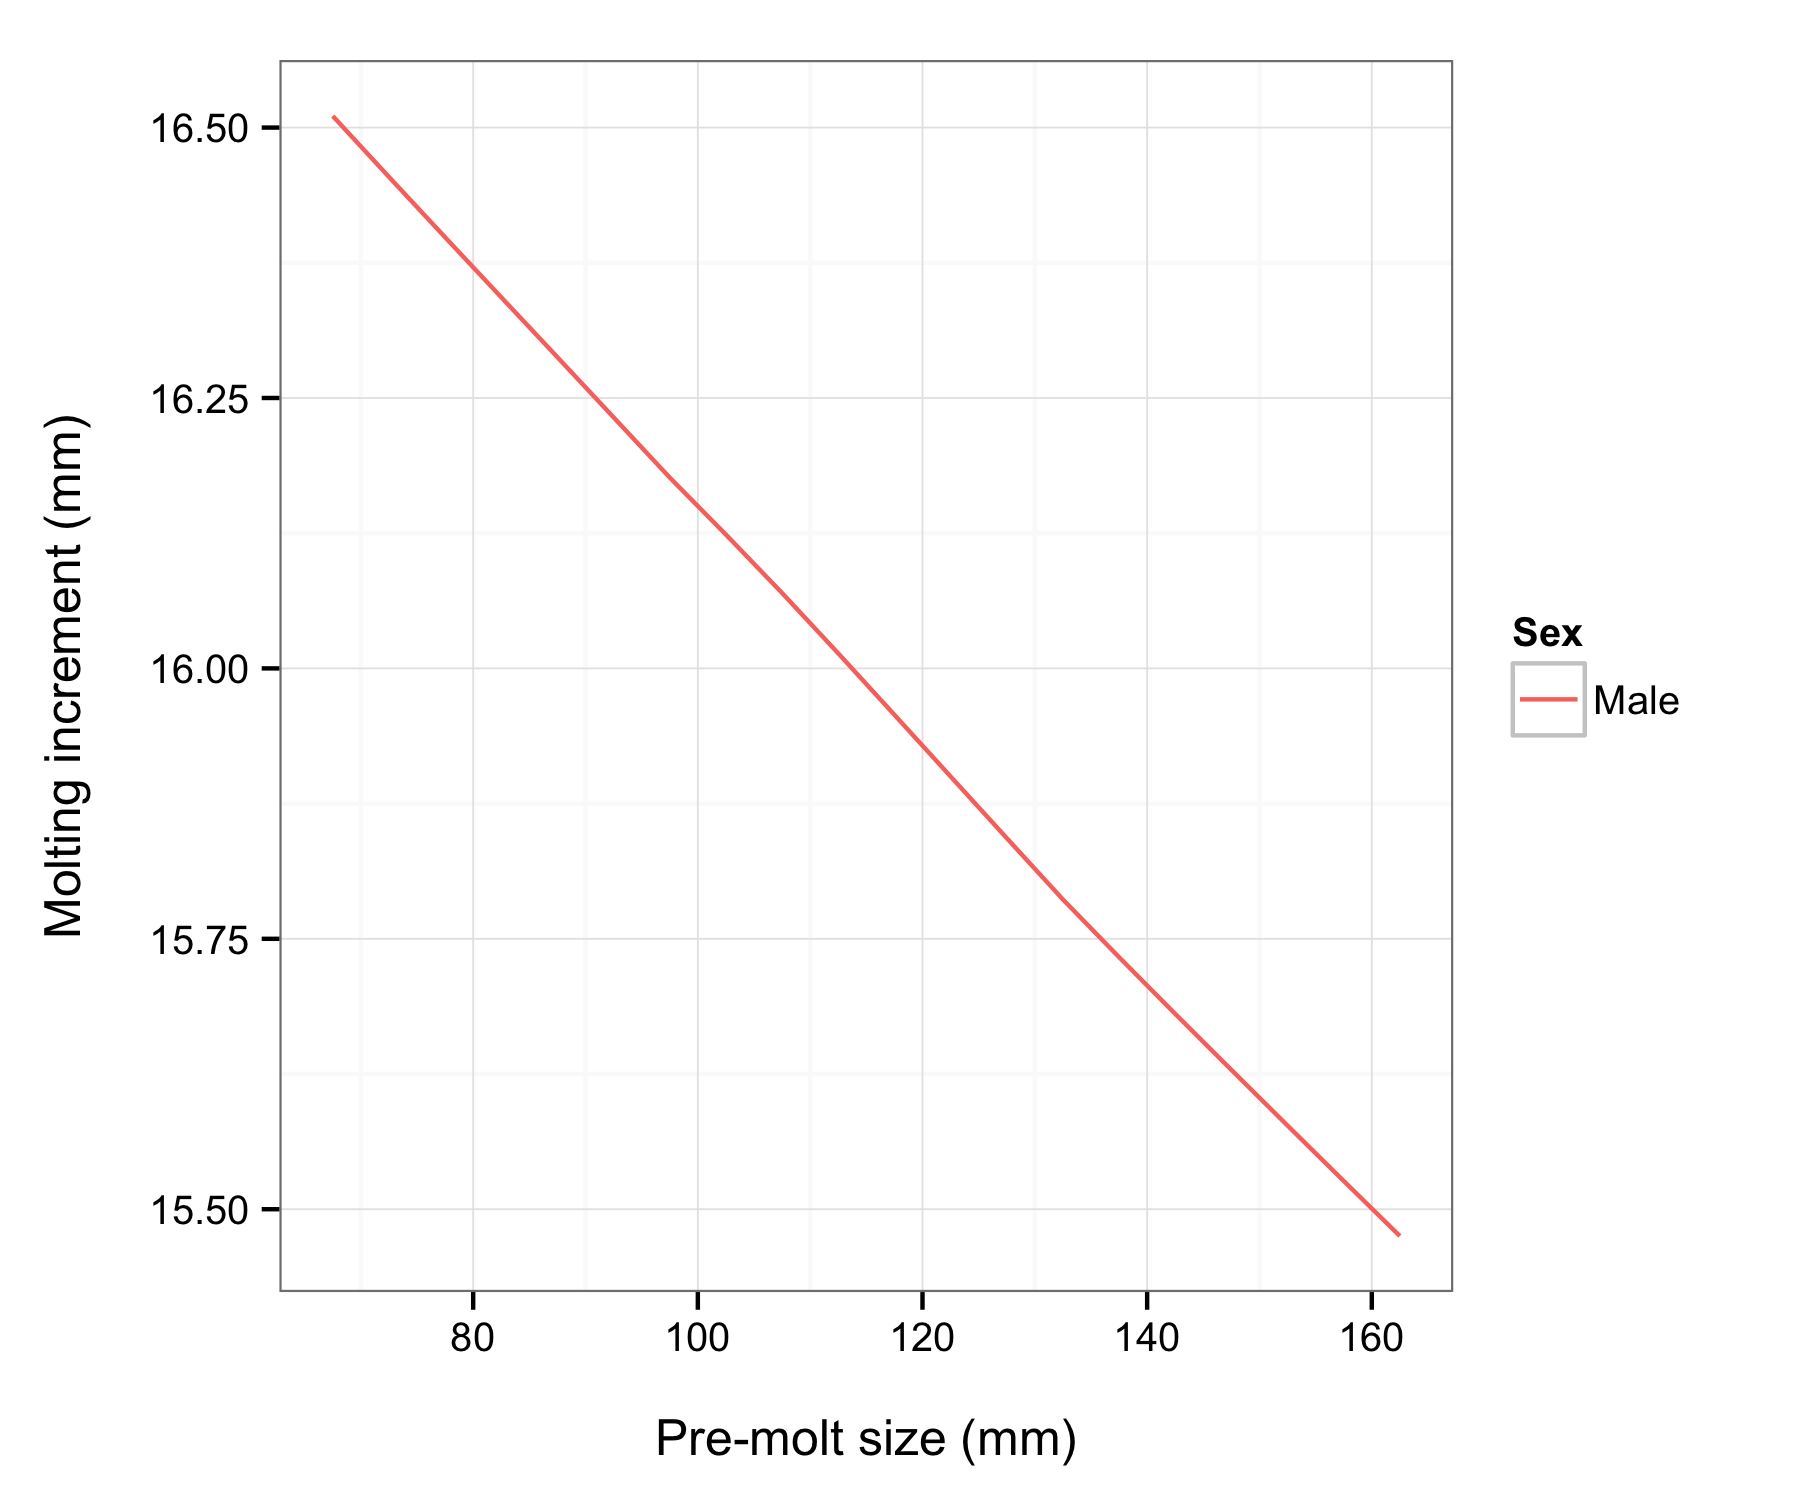
\includegraphics[width=0.75\linewidth]{../../examples/bbrkc/OneSex/figure/gi.png}
\end{figure}
\end{frame}

%% =========================================================================== %%

\begin{frame}
\frametitle{Growth}
Growth transition
\begin{figure}[!htbp]
  \centering
  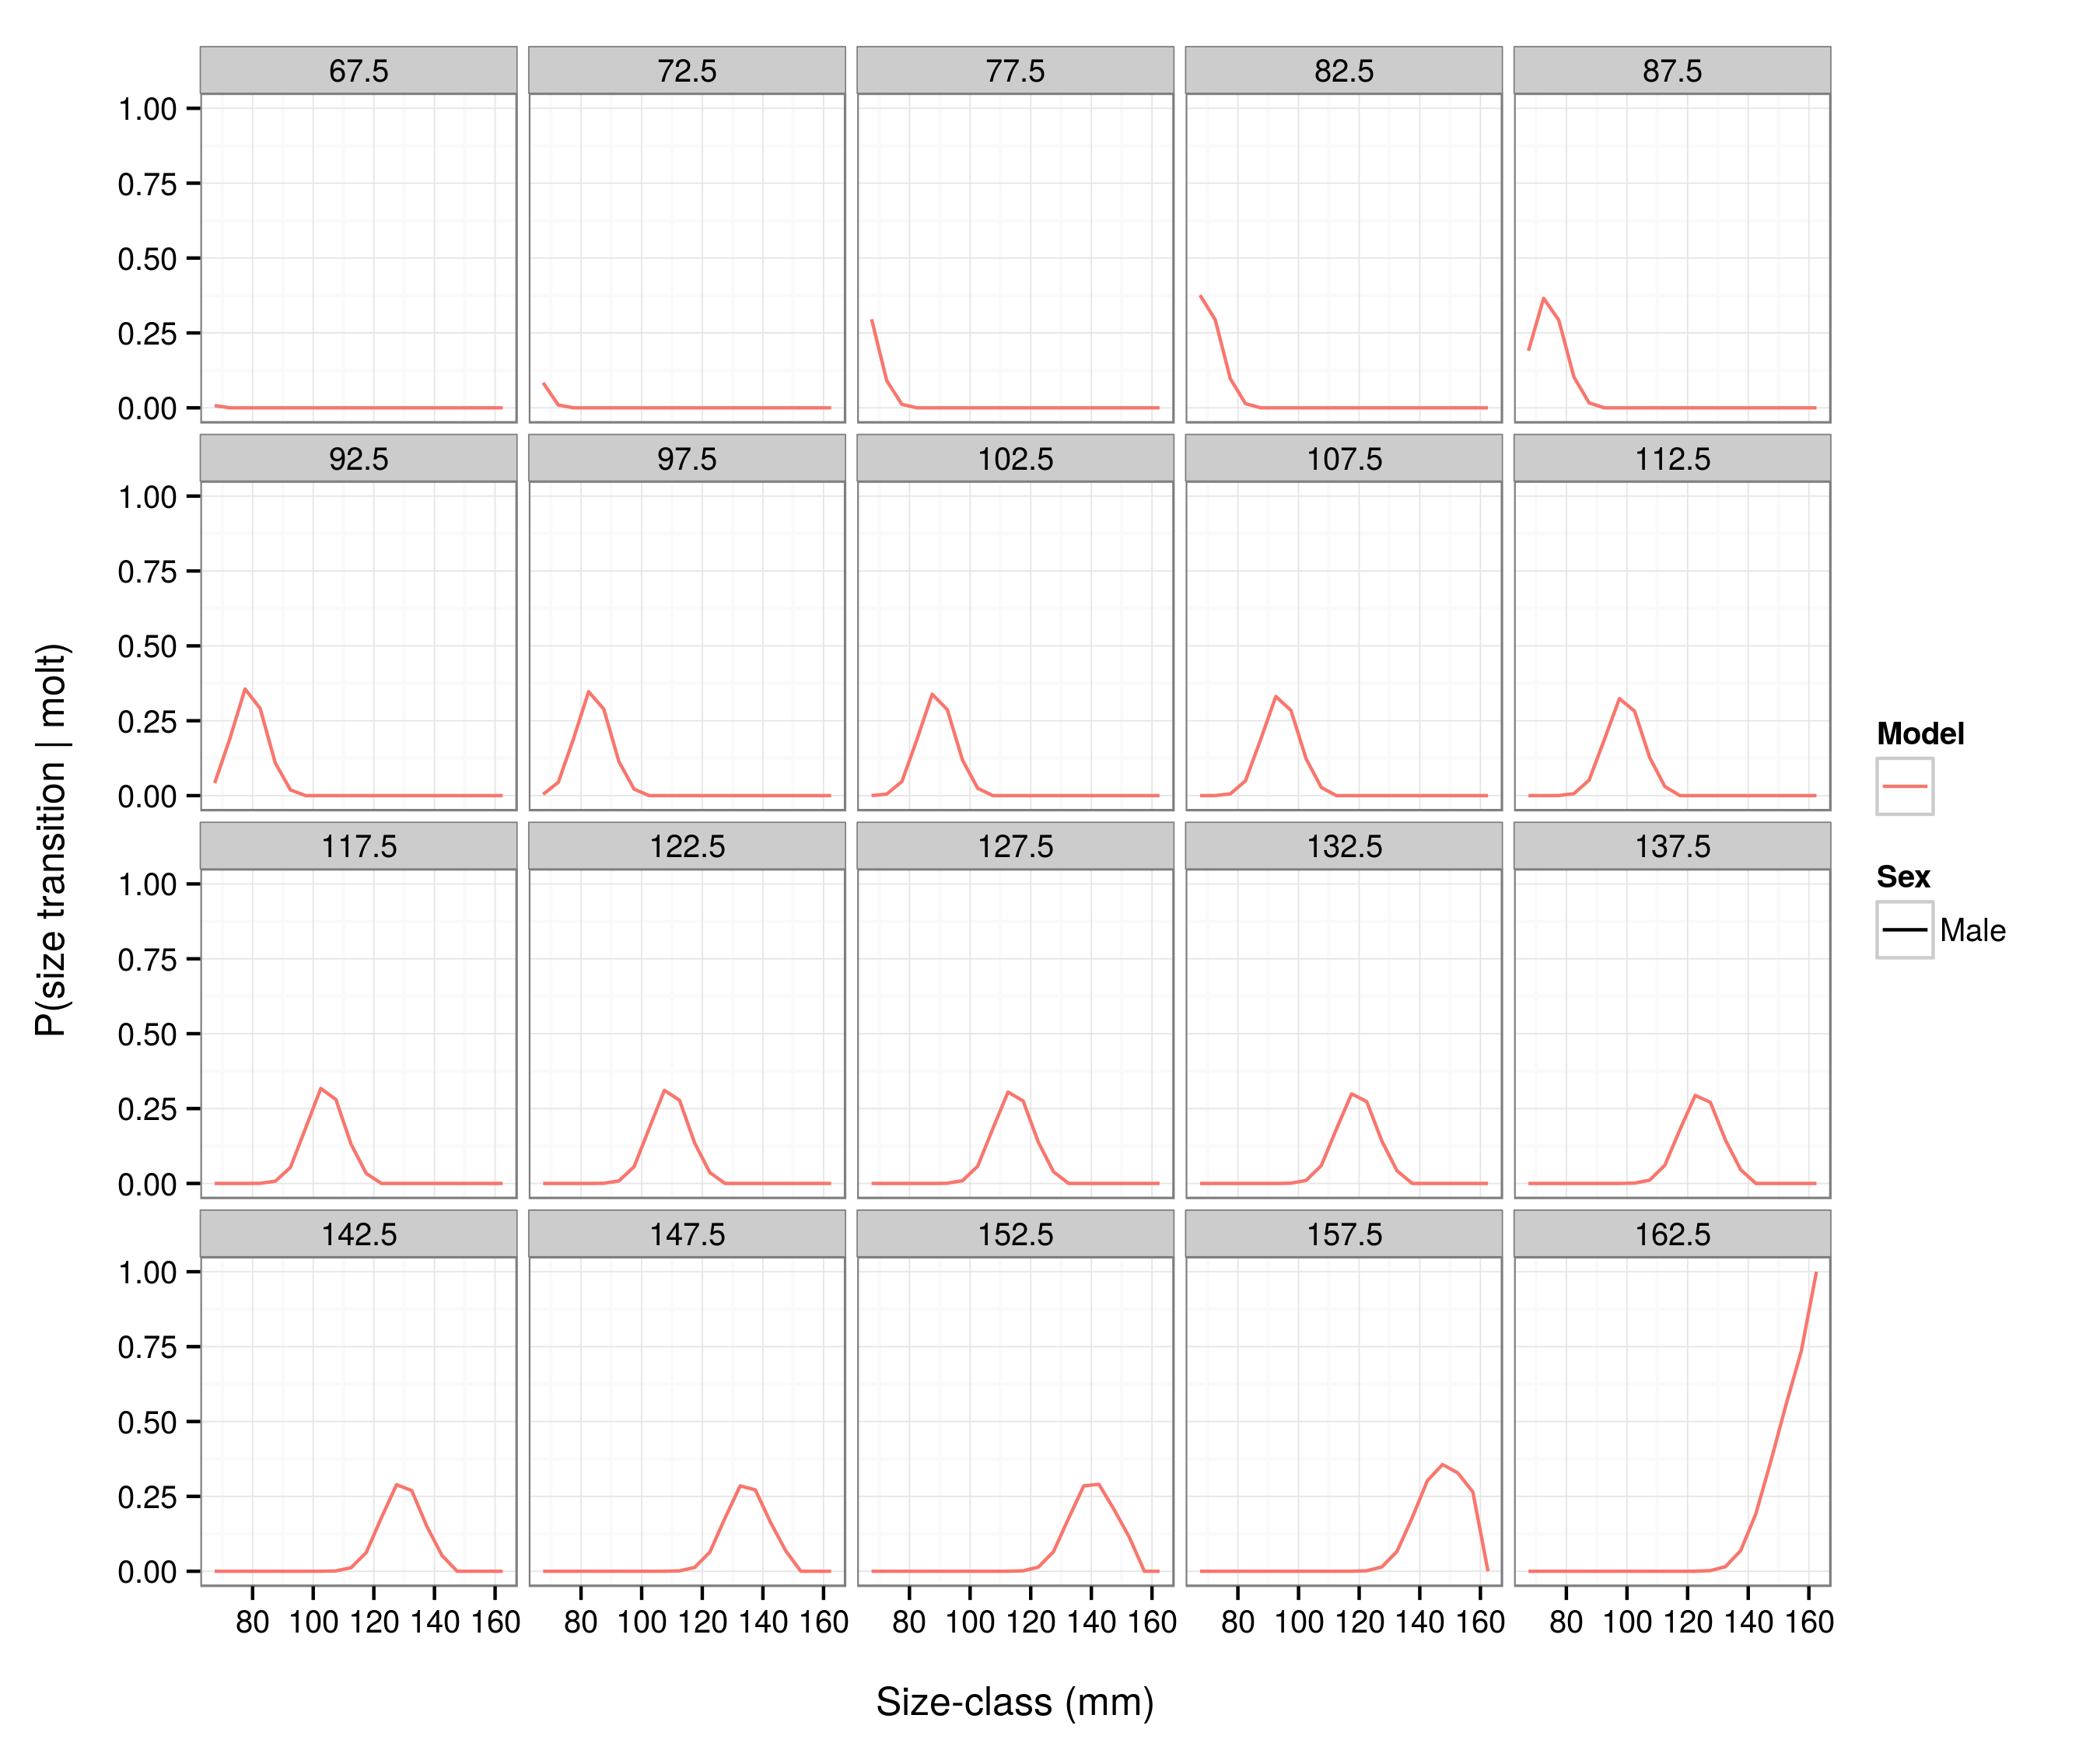
\includegraphics[width=0.75\linewidth]{../../examples/bbrkc/OneSex/figure/growth_transition.png}
\end{figure}
\end{frame}

%% =========================================================================== %%

\subsection{Natural mortality}
\begin{frame}
\frametitle{Natural mortality}
Natural mortality ($M$) is assumed to be sex-specific ($h$), size-independent
($\ell$), and may or may not be constant over time ($i$). If time-varying
natural mortality is used, the model constrains $M_{h,i}$ to be a random-walk
process with variance $\sigma^2_M$
\begin{equation*}
  M_{h,i+1} = 
  \begin{cases}
    \bar{M}_h\\
    M_{h,i} e^{\delta_i}
  \end{cases},
\end{equation*}
where
\begin{equation*}
  \delta_i \sim \mathcal{N} \left( 0, \sigma^2_M \right).
\end{equation*}
A time-varying natural mortality can be estimated for all years ($i$), or for
specified blocks of years ($\iota \in i$).
\end{frame}

%% =========================================================================== %%

\begin{frame}
\frametitle{Natural mortality}
Assuming natural mortality is time-varying constrained by variance ($\sigma^2_M
= 0.04$) at four specific knots (1976, 1980, 1985, 1994)
\begin{figure}[!htbp]
  \centering
  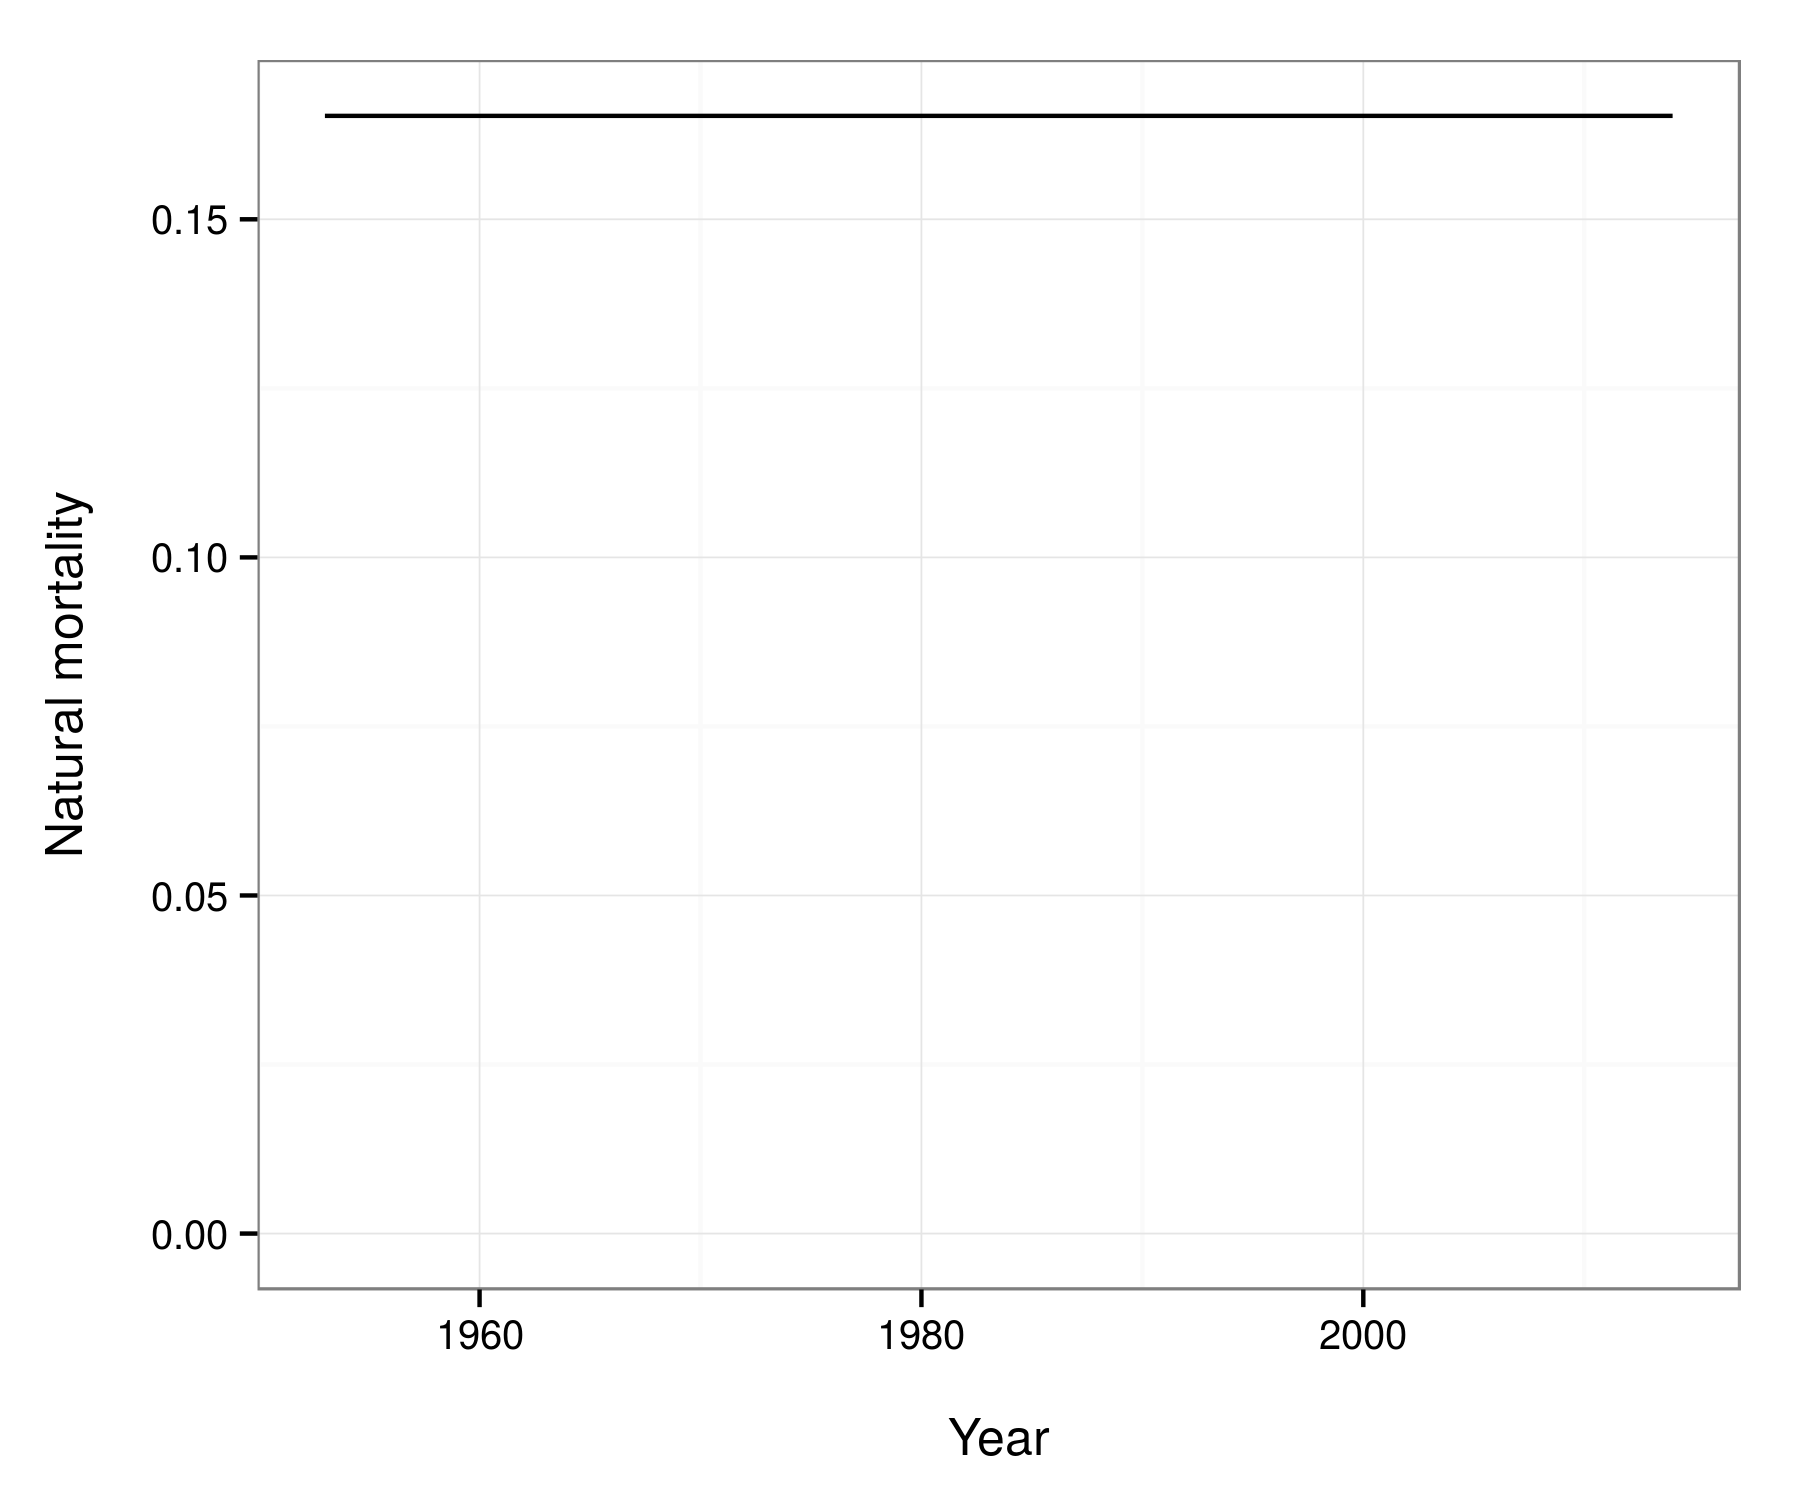
\includegraphics[width=0.65\linewidth]{../../examples/bbrkc/OneSex/figure/M_t.png}
\end{figure}
\end{frame}

%% =========================================================================== %%

\begin{frame}
\frametitle{Selectivity and retention}

The probability of catching an animal of sex $h$, in year $i$, in fishery $k$,
of length $\ell$ (i.e. selectivity) is
\begin{equation*}
  s_{h,i,k,\ell} = (1 + \exp(-(\ell-a_{h,i,k})/\sigma_{h,i,k}^s))^{-1}.
\end{equation*}

The probability of an animal of sex $h$, in year $i$, in fishery $k$, of length
$\ell$ being reatained is
\begin{equation*}
  y_{h,i,k,\ell} = (1 + \exp(-(r_{h,i,k}-\ell)/\sigma_{h,i,k}^y))^{-1}.
\end{equation*}

The joint probability of vulnerability due to fishing mortality and discarding
is
\begin{equation*}
  \nu_{h,i,k,\ell} = s_{h,i,k,\ell} \left[ y_{h,i,k,\ell} + (1 - y_{h,i,k,\ell})
    \xi_{h,k} \right],
\end{equation*}
where $\xi_{h,k}$ is the discard mortality rate for sex $h$ in fishery
$k$.
\end{frame}

%% =========================================================================== %%

\begin{frame}
\frametitle{Selectivity and retention}
Assuming that selectivity for the NMFS trawl fishery is split into two blocks
(1975-1981 and 1982-2014) and that retention is constant with time
$y_{h,i,k,\ell} = y_{h,k,\ell}$
\begin{figure}[!htbp]
  \centering
  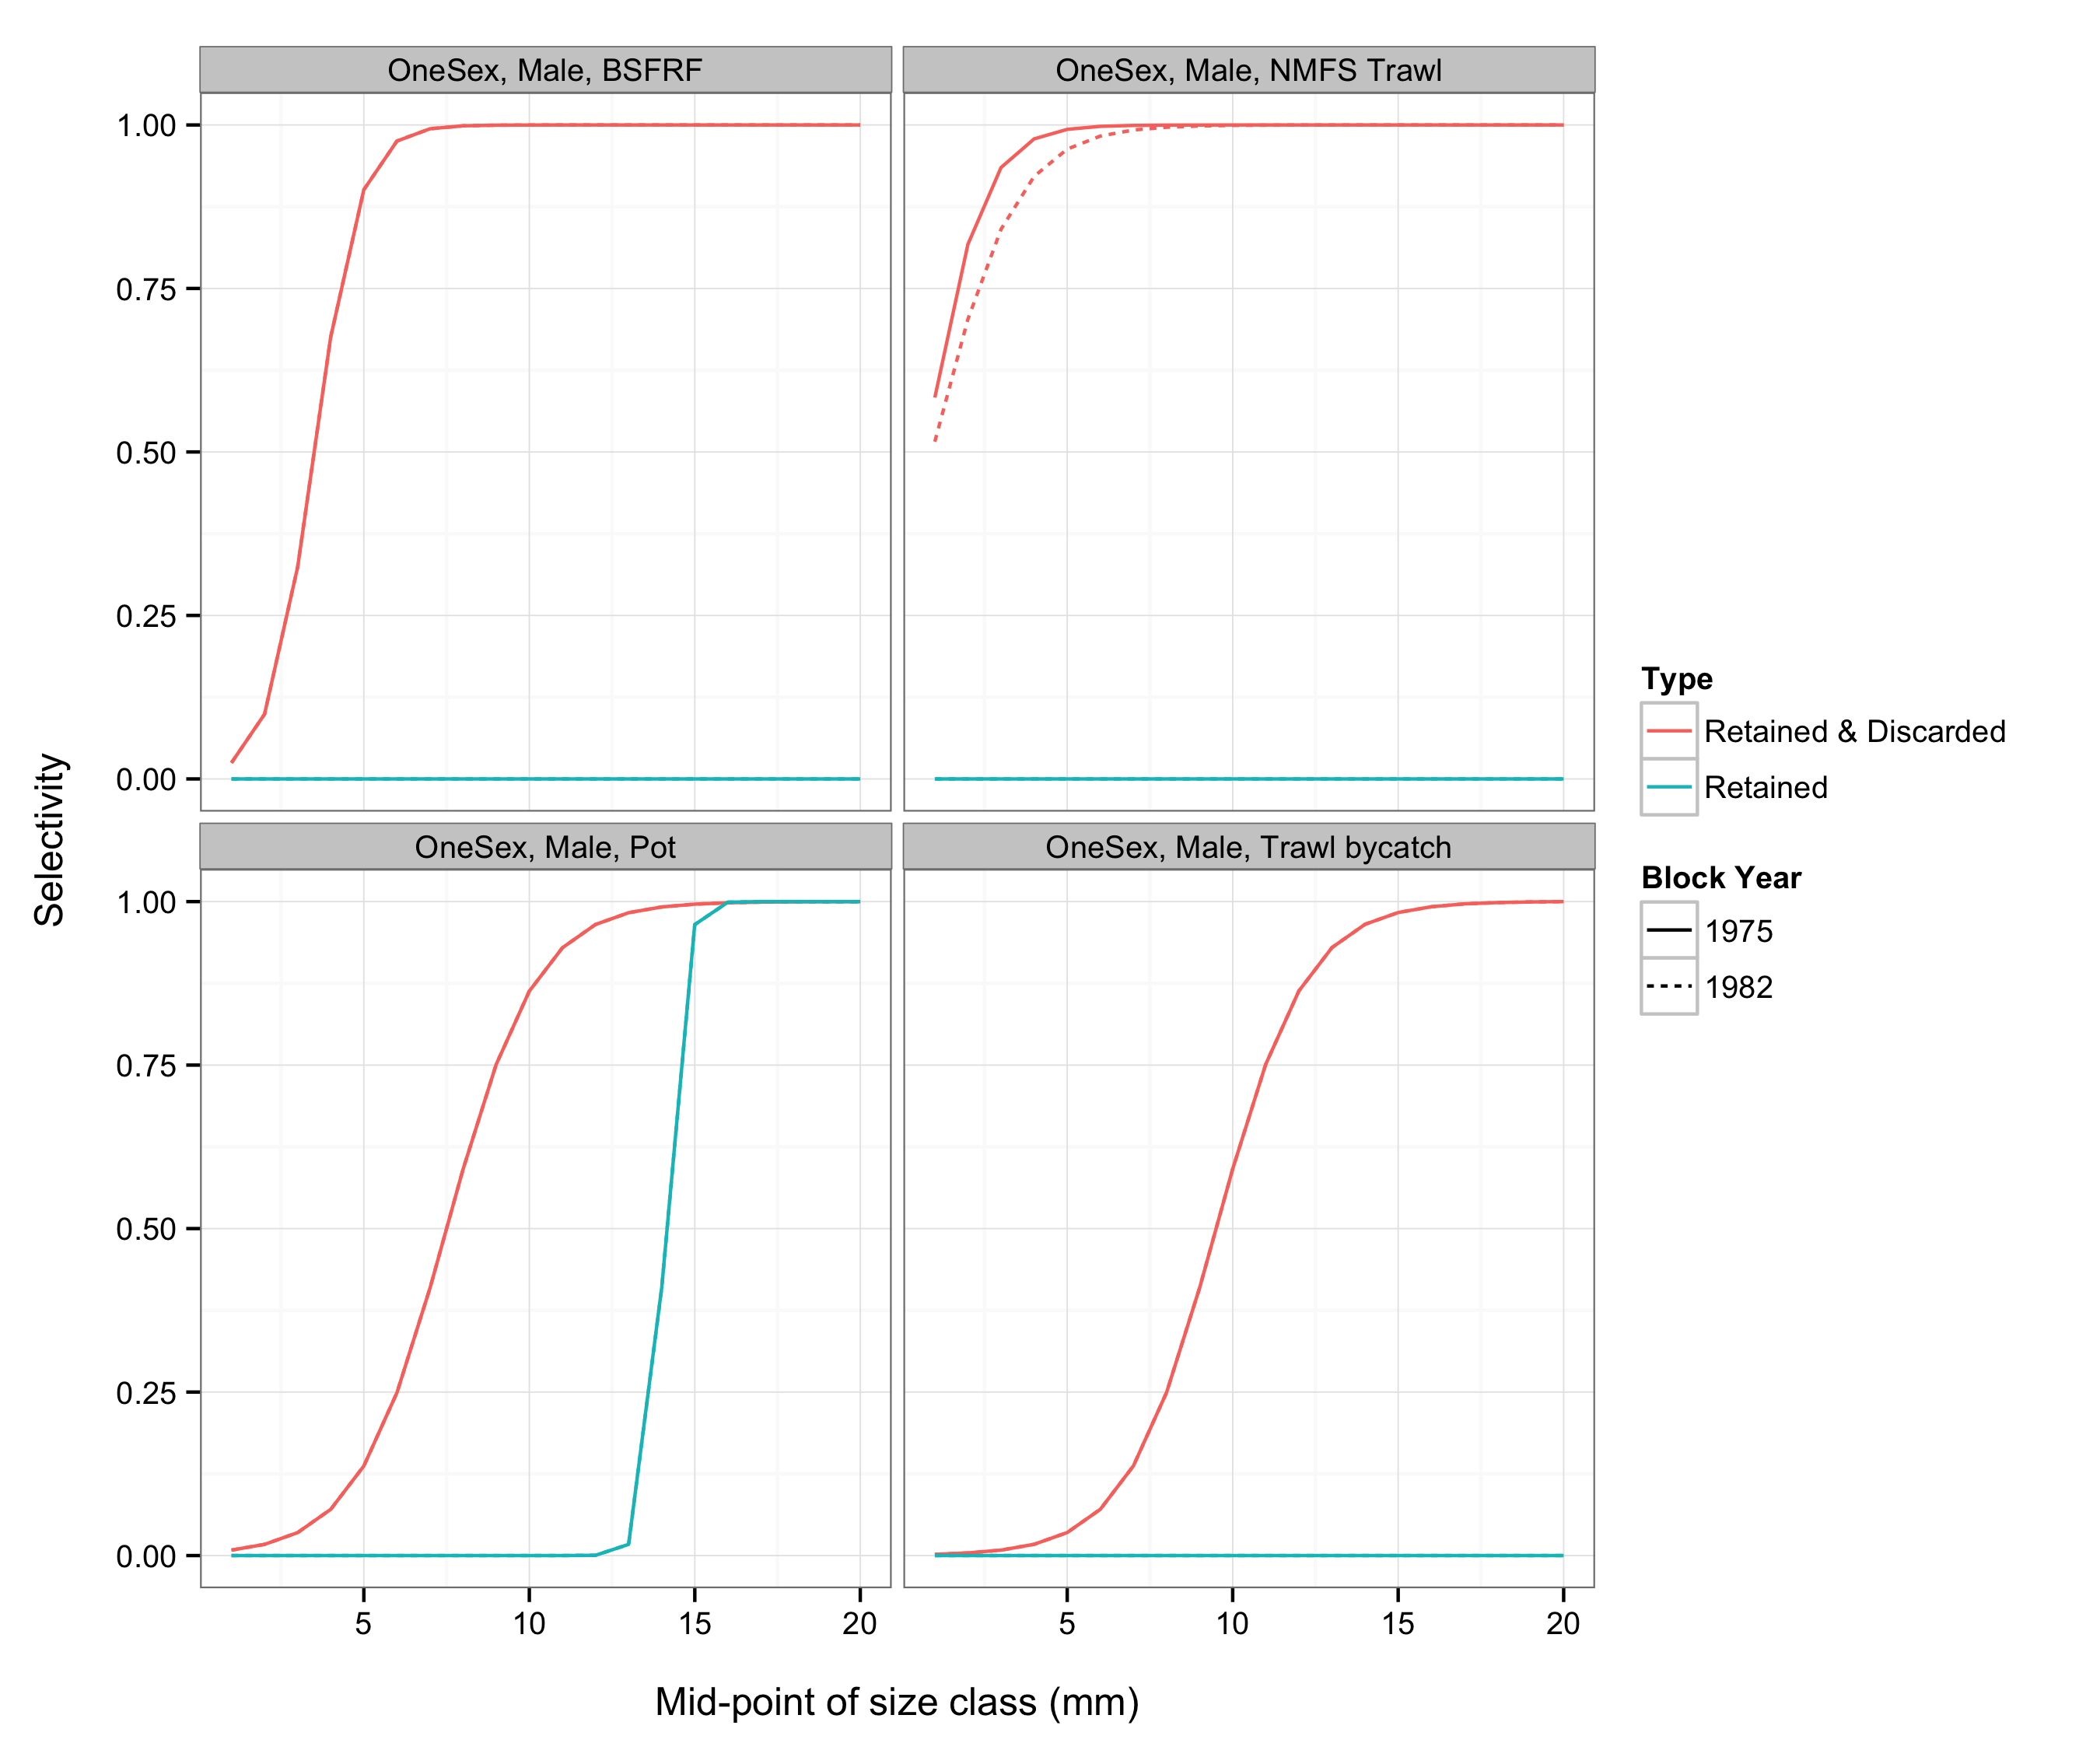
\includegraphics[width=0.6\linewidth]{../../examples/bbrkc/OneSex/figure/selectivity.png}
\end{figure}
\end{frame}

%% =========================================================================== %%

\begin{frame}
\frametitle{Fishing mortality}
\begin{align*}
  \boldsymbol{F}_{k,i} &= \exp \left( \bar{\boldsymbol{f}}_k + \Psi_{k,i}
  \right),\\
  \boldsymbol{f}_{h,i} &= \sum_k \boldsymbol{F}_{k,i} \nu_{h,i,k,\ell},
\end{align*}
\end{frame}

%% =========================================================================== %%

\subsection{Growth and survival}
\begin{frame}
\frametitle{Growth and survival}
Growth and survival
\begin{equation*}
  \boldsymbol{A}_{h} = \boldsymbol{G}_h \left[ \exp (-\bar{M}_h) \boldsymbol{I}
  \right].
\end{equation*}
Growth and survival including fishing mortality
\begin{equation*}
  \boldsymbol{B}_{h,i} = \boldsymbol{G}_h \left[ \exp (-M_{h,i} -
    \boldsymbol{f}_{h,i}) \boldsymbol{I} \right].
\end{equation*}
\end{frame}

%% =========================================================================== %%

\section{Steady-state conditions}
\subsection{Survivorship to length}

\begin{frame}
\frametitle{Survivorship to length}

Survivorship to length
\begin{align*}
  \boldsymbol{u}_h &= -(\boldsymbol{A}_h - \boldsymbol{I})^{-1} (p(\boldsymbol{r})),\\
  \boldsymbol{v}_h &= -(\boldsymbol{B}_h - \boldsymbol{I})^{-1} (p(\boldsymbol{r})).
\end{align*}

Steady-state conditions
\begin{align*}
  B_0 &= R_0 \sum_h \lambda_h \sum_\ell \boldsymbol{u}_h w_{h,\ell} m_{h,\ell},\\
  \tilde{B} &= \tilde{R} \sum_h \lambda_h \sum_\ell \boldsymbol{v}_h w_{h,\ell}
  m_{h,\ell}.
\end{align*}
\end{frame}

%% =========================================================================== %%

\begin{frame}
\frametitle{Recruitment}

Recruitment size-distribution
\begin{align*}
  \alpha &= \frac{\alpha_r}{\beta_r},\\
  p(\boldsymbol{r}_i) &= \int^{x_\ell+0.5 \Delta x}_{x_\ell-0.5 \Delta x}
  \frac{x^{\alpha-1} \exp
    \left(\frac{x}{\beta_r}\right)}{\Gamma (\alpha) x^\alpha} dx,\\
  \boldsymbol{r}_{h,i} &= 0.5 p(\boldsymbol{r}_i) \ddot{R}.
\end{align*}

\end{frame}

%% =========================================================================== %%

\begin{frame}
\frametitle{Population dynamics}

Initial numbers at length
\begin{equation*}
  \boldsymbol{n}_{h,i} = \left[-\left( \boldsymbol{A}_{h} - \boldsymbol{I}
    \right)^{-1} \boldsymbol{r}_{h,i} \right] e^{\boldsymbol\nu} \quad
  \text{where} \quad i=1.
\end{equation*}

The numbers in each size-class in the following time-step
($\boldsymbol{n}_{h,i+1}$) is the product of the numbers in each size-class in
the previous time-step ($\boldsymbol{n}_{h,i}$), size-specific growth and
survival ($\boldsymbol{A}_{h,i}$), plus new recuits ($\boldsymbol{r}_{h,i}$)
\begin{equation*}
  \boldsymbol{n}_{h,i+1} = \boldsymbol{n}_{h,i} \boldsymbol{A}_{h,i} +
  \boldsymbol{r}_{h,i} \quad \text{where} \quad i > 1.
\end{equation*}



\end{frame}

%% =========================================================================== %%

\begin{frame}
\frametitle{Outline}
\tableofcontents
\end{frame}

%% =========================================================================== %%

\begin{frame}
\frametitle{Outline}
\tableofcontents
\end{frame}

%% =========================================================================== %%

\begin{frame}
\frametitle{Outline}
\tableofcontents
\end{frame}

%% =========================================================================== %%

\begin{frame}
\frametitle{Outline}
\tableofcontents
\end{frame}

%% =========================================================================== %%

\begin{frame}
\frametitle{Data weighting}

Log-likelihood, likelihood, distribution
\begin{align*}
  \ell (\mu, \sigma^2, \lambda; x) &= \lambda \left( -\frac{1}{2} \log (2 \pi) - \frac{1}{2}
  \log (\sigma^2) - \frac{1}{2 \sigma^2} (x - \mu)^2 \right)\\
  p(x|\mu, \sigma^2, \lambda) &= \exp(\lambda) \left( 2 \pi \sigma^2 \right)^{-\frac{1}{2}} \exp \left[ -\frac{1}{2
      \sigma^2} (x - \mu)^2 \right]\\
  x|\mu, \sigma^2, \lambda &\sim \mathcal{N} \left( \mu, \lambda \sigma^2 \right)
\end{align*}
\end{frame}

%% =========================================================================== %%

\end{document}